\chapter{Introducción}
%%---------------------------------------------------------

Esta idea surgió a raíz de una práctica de programación impartida por la universidad.

En Programación I, asignatura que se cursa en el primer año del grado, se propuso como ejercicio de final de la asignatura un proyecto en lenguaje Java de tema libre en equipos de dos personas. Nos unimos una compañera de clase, Andrea del Nido, y yo. 

Al principio no contábamos con tanta experiencia y no fue fácil encontrar un tema interesante. Sin embargo, ante el movimiento general de toda la clase por hacer un videojuego (hundir la flota, adivina el número), decidimos seguir el camino de crear un programa de un juego, pero tampoco se nos ocurría una alternativa a los proyectos de nuestros compañeros.

Entonces una compañera de clase nos propuso la idea de un juego de pistas, es decir, un juego de buscar objetos para luego poder usarlos en otro lugar, añadiéndole una historia bien definida y atractiva.

\begin{figure}[h]
	\caption{Ejemplo de una ejecución del juego}
	\centering
	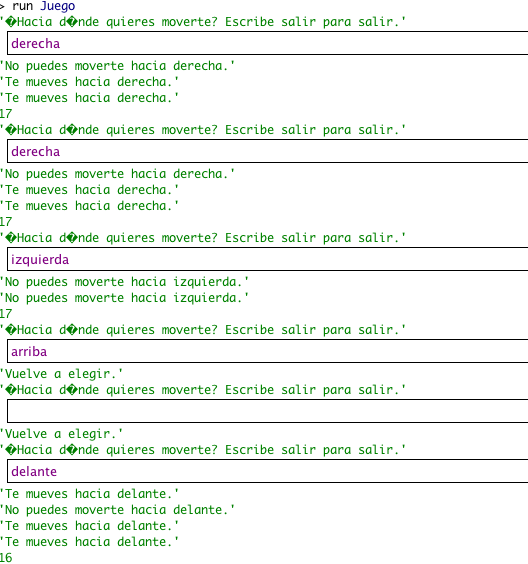
\includegraphics[width=0.75\textwidth]{include/primerJuegoCaptura.png}
\end{figure}

Así nos pusimos manos a la obra a desarrollar esa idea y la historia que conllevaba. Como era un proyecto complejo para nuestro nivel de aprendizaje en el momento y además muy alejado de las prácticas de programación, llevamos a cabo una lluvia de ideas de todas las cosas que podría incluir el proyecto, intentando ser muy ambiciosos para luego poder descartar opciones.
Personalmente me involucré mucho en el desarrollo ya que me encantan los videojuegos y además siempre había querido trabajar en un proyecto de este tipo.

Tras muchas horas extra de programación, conseguimos una primera versión funcional sin muchos errores para la presentación del proyecto. Se hablará de cómo funcionaba el juego en el próximo apartado.

A partir de ahí, tras pedir permiso a mi compañera para continuar con el desarrollo por mi cuenta, proseguí arreglando errores del proyecto para tener una versión aceptable para jugar.
Así pasaron los dos años siguientes del grado, dando en cada semestre una nueva asignatura de programación que aunque no estuvieran centrados en continuar este proyecto, me permitieron ir mejorando ciertas implementaciones del juego así como añadir ciertas funcionalidades que no estaban presentes desde un principio.

Poco a poco, sin embargo fui dejando el proyecto en el olvido debido a una mezcla de falta de tiempo por estudios y prácticas y también por falta de nuevas ideas, ya que la ártifice de las grandes ideas del proyecto era mi compañera.

En el último año del grado, tras enterarme de que se podría presentar un proyecto con un tema personalizado pensé inmediatamente en continuar con el desarrollo de Historias del Laberinto.
Con la ayuda de Andrea del Nido y Andrea de las Heras, llegamos a la conclusión de que no podía presentar lo que llevaba hecho hasta el momento, porque todas las actualizaciones y mejoras que fui programando provocaron que el código fuera muy difícil de modificar.
Además el juego era muy difícil de mostrar, ya que necesitaba de una máquina virtual Java para reproducirse y mucha gente cercana me preguntó si este juego se podía jugar en el móvil.

Por lo tanto, el tema se centraría en el desarrollo de un nuevo videojuego que permitiría al usuario jugarlo en un dispositivo móvil, que contara con un sistema genérico de desarrollo de eventos, así como las características del juego original.

Inicié la búsqueda del tutor que pudiera llevar el trabajo, y por suerte encontré a mi actual tutor, Ángel Herranz, al que le doy las gracias por permitirme desarrollar este proyecto.
Él se interesó desde el principio en la idea del proyecto, y me sugirió varias pautas para llevar el trabajo con él.

\newpage
\section{Qué era antes Historias del Laberinto}

Esta sección se centrará en la explicación de lo que fue Historias del Laberinto durante su desarrollo como proyecto de Programación I y sus mejoras posteriores.
Primero se hablará de los aspectos relacionados con el primer proyecto.

El proyecto original era una aplicación capaz de reproducir una historia única sobre dos personajes, Gerar y el jugador, al que se le podía poner un nombre.

La trama del juego sigue un argumento parecido a muchos juegos de escape: los dos personajes debían escapar del Laberinto, un misterioso lugar lleno de trampas del que no saben cómo llegaron ni cómo pueden salir. Por ello, el jugador y su compañero debían avanzar por las salas del laberinto hasta llegar a la sala final, donde un malvado dragón les separaba de su esperada salida. Durante el camino encontrarán carismáticos personajes como el Fantasma, salas del tesoro, encuentros con monstruos o salas con truco.

Respecto a la funcionalidad, tras la lluvia de ideas sobre lo que el juego debía de ser capaz de hacer, se desarrollaron los siguientes subsistemas principales: menú de juego, movimiento, inventario, combate y pantalla de carga. Aparte se incluían otras funcionalidades extra.
A continuación se describirá un poco qué hacía cada uno de ellos.

\begin{figure}[h]
	\caption{Gerardo, el compañero del videojuego}
	\centering
	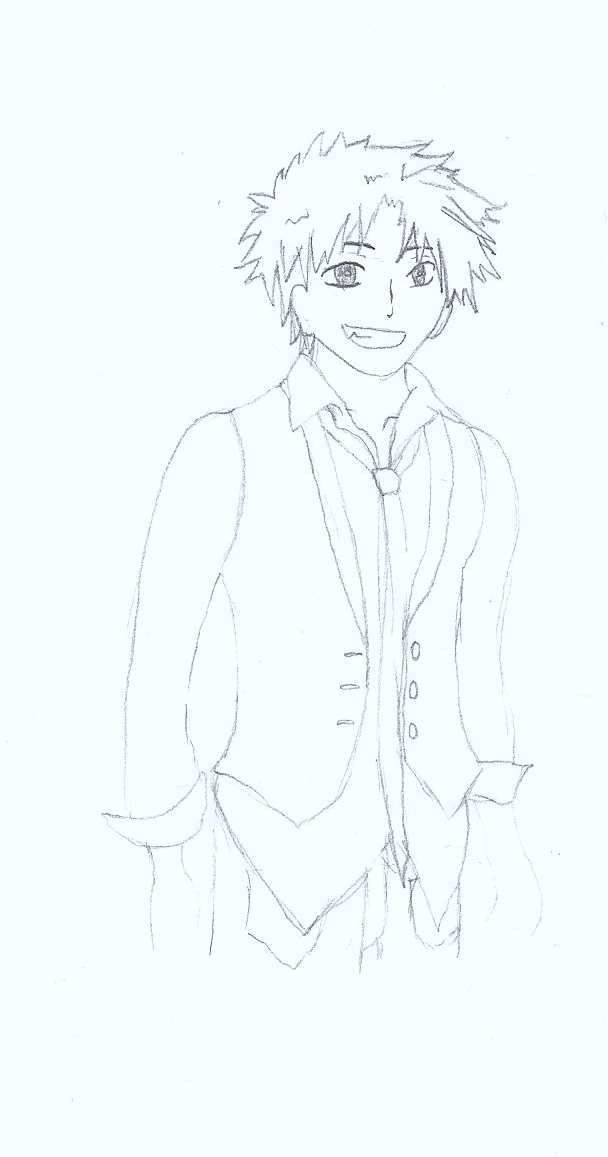
\includegraphics[width=0.25\textwidth]{include/GerardoPres.png}
\end{figure}

\subsection{Menú de juego}

El juego se pensó desde un principio como un sistema simple que incluía lo que en otros cursos llamaríamos estados  y un bucle de ejecución que evaluaba estos estados y generaba los eventos necesarios.

Este sistema consistía en un bucle que siempre mostraba las mismas opciones: hablar, interactuar, inventario y moverse. Estas acciones cambiaban según una serie de parámetros que definían el estado de ejecución del programa: un número que indicaba una sala, un valor booleano que decía si el compañero estaba jugando y un mapa de lugares ya visitados.

\subsection{Siguiente paso}

En el desarrollo inicial del juego, toda la salida de la interfaz y los diálogos era por consola, por lo que todos los diálogos que ocurrían en la historia se imprimían por consola.

Debido a la rapidez de la ejecución de las instrucciones, las líneas de código que se encargaban del diálogo eran directamente impresas en consola y se ejecutaban muy rápidamente, provocando que al pulsar una acción o una respuesta, todo el texto siguiente apareciera rápidamente en consola  y muchas veces fuera ilegible.

Por ello se pensó en una funcionalidad que esperaba ante una respuesta del usuario cualquiera, normalmente un pulsado de la tecla "\textit{intro}", para mostrar el siguiente diálogo y hacer posible que la ejecución del juego fuera más legible.

\subsection{Pantalla de carga}

El funcionamiento del juego en la aplicación era muy rápido, aunque la calidad del código no fuera óptima. Los conceptos adquiridos en la asignatura nos introdujeron en ámbitos básicos del lenguaje de programación Java, por lo que las operaciones que se llevaban a cabo siempre eran muy rápidas. Además, ninguna operación dependía de otra, no contaba con concurrencia, no hacía conexiones con Internet ni se encargaba de parsear  información antes de ejecutar el núcleo del juego.

Debido a que no había ningún recurso que cargar ni inicializar, el juego se iniciaba instantáneamente.
Aunque esto puede ser positivo para un programa, nosotros creímos en su momento indispensable separar ciertas funcionalidades del juego como el inicio, una batalla, un evento del resto para intentar emular una característica que aparece en todos los juegos actuales: la pantalla de carga.

Esta funcionalidad simplemente paraba el hilo de ejecución cada cierto tiempo y mientras tanto iba imprimiendo por consola un mensaje que indicaba que la aplicación estaba cargando.

\subsection{Movimiento}

La función de movimiento permitía a un jugador moverse entre las salas del laberinto. Para ello, se pensó en un mapa de posiciones, de manera que cada posición representara una habitación.
Cada sala estaba representada como un número del 1 al 20, y cada uno de estos números se ubicaron en un mapa, representado como una matriz de 5 columnas y 4 filas que recogía la información de la sala que se ubicaba en cada casilla. Todas las salas eran diferentes entre sí.

De esta manera se deducía que la posición actual de un jugador y las posiciones de cada sala estaban dadas por unas coordenadas que representaban los índices legales para la matriz, es decir, índices para que no surja un error al intentar acceder a la información de la matriz del mapa. Las coordenadas que se usaban eran una para la primera matriz, que representaba como el eje de la x, y otra para las submatrices de la primera matriz, que representaba como el eje de la y.

Un jugador tiene cuatro opciones para moverse: ir hacia delante, hacia atrás, a la derecha o a la izquierda. Al seleccionar una dirección, el sistema calculaba si ese movimiento era posible y lo ejecutaba.
Todo esto incluía como un extra un sistema de direcciones mediante el uso de una brújula. Esto significa que al moverse a cualquier dirección que no fuera adelante se cambiaba la dirección hacia la que estaba mirando el grupo. De esta manera el jugador estaba siempre mirando a alguno de los puntos cardinales, y calculaba el movimiento teniendo en cuenta la dirección escogida.

Este sistema era capaz de evitar que al moverse el jugador pudiera irse fuera de los límites de la matriz y también de evitar el movimiento hacia ciertas salas desde ciertos lados.

\subsection{Inventario}

La función del inventario está pensada como un sistema de uso de objetos. Incluye un gestor de objetos y un menú de uso de los objetos.

En el proyecto original, la idea principal para manejar los objetos contaba con que solo el protagonista podía tener un inventario, es decir, una referencia a los objetos conseguidos y guardados. De esta manera, solo el protagonista podía conseguir objetos y usarlos, aunque posteriormente se añadió funcionalidad para que el compañero pueda usarlos también.

Existían dos tipos de objetos genéricos: consumibles y objetos clave. 
Los consumibles son objetos que se pueden consumir por el protagonista o el compañero y que modifican el valor de los puntos de vida actuales de los personajes. Un ejemplo de un objeto consumible es una poción, que recuperaba una cantidad de puntos de vida actuales.
Los objetos clave son objetos que solo pueden usarse fuera de las batallas en ciertas salas del laberinto y que suelen activar eventos. Son objetos que además no se pueden usar dentro de una batalla, y por lo tanto al usarlos mostraban un diálogo con una descripción del objeto.

Los dos tipos de objetos son limitados, es decir, hay una cantidad reducida de los mismos por partida y además al usarse se gastan, por lo que podría llegar un momento en el juego en que no quedaran objetos.

\subsection{Combate}

El combate se presentó como un sistema genérico de combate que incluía tres posibles actores: el protagonista, el compañero y un enemigo. El protagonista y el compañero formaban un equipo y se enfrentaban al enemigo, que podía ser un personaje genérico cualquiera.

El combate siempre giraba alrededor de los puntos de vida actuales del enemigo y del protagonista, por lo que si alguno de estos llegaba al cero entonces el combate se terminaba.

El sistema de combate es un combate por turnos del estilo de juegos de rol (RPG) como los descritos en la introducción, es decir, un sistema de combate por turnos, siguiendo un orden fijo preestablecido:
\begin{enumerate}
	\item Protagonista
	\item Enemigo
	\item Compañero
\end{enumerate} 
	
Siempre siguiendo este orden de actuación en los turnos, cada turno tenía una serie de fases bien fijadas:
\begin{enumerate}
	\item Cálculo de daño inicial: permitía calcular si el siguiente turno debía ejecutarse o no, según si el actor que fuera a actuar tuviera más de cero puntos de vida actuales.
	\item Selección de acción y objetivo: dependiendo del personaje, se podían realizar ciertas acciones. En el caso del protagonista, el personaje controlado por el jugador, existían tres opciones: atacar, estado e inventario. El enemigo siempre usa el comando Atacar y se elige aleatoriamente el objetivo del ataque. El compañero podía elegir entre atacar o usar el inventario según ciertos parámetros, cómo la vida restante.
	\item Resolución de daño: tras haber atacado a un objetivo, se calculan los puntos de vida restantes del objetivo del ataque y se calcula si la batalla ha de terminar o si debe continuar. La batalla terminaba si el protagonista o el enemigo eran derrotados.
\end{enumerate} 
	
En desarrollos posteriores a la entrega del primer trabajo, se incluyó la posibilidad de que un personaje del combate pudiera tener un estado alterado de una lista fija: envenenado, paralizado y ciego.
Esto permitía hacer más diverso el combate, ya que impedía a un jugador no actuar o provocaba que fallara siempre los ataques.

\section{Por qué un intérprete de videojuegos}

Antes de empezar con la razón detrás de esta elección, querría hablar un poco de los tipos de juegos. A mi parecer, existen dos tipos de juegos: los juegos que se centran en contar una historia y los que se centran en desarrollar una jugabilidad entretenida o rompedora. Aunque es cierto que muchas veces estos dos tipos de juegos se entrelazan, pocos son los que se puede decir que tengan una jugabilidad amena y con una historia que no solo sea atractiva para un jugador, sino que esté intimamente relacionada con el juego en sí.

Para mostrar este hecho, pongamos algunos ejemplos:

\begin{itemize}
	\item Final Fantasy: esta saga de videojuegos tienen todos un núcleo común, una historia que se desarrolla a lo largo de todo el videojuego. Normalmente se resume en un grupo de compañeros que viajan por todo su mundo para salvar de algún malvado. El foco principal de estos videojuegos es la historia que tienen que contar.
	\item Super Smash Bros: sin embargo esta otra saga, aunque alguna de sus entregas cuenta con historia, se centra en su jugabilidad principal: combates a tiempo real entre personajes de Nintendo, como Mario, Luigi... Este juego no tiene una historia muy atractiva, y no se centra en avanzarla a lo largo del juego.
	\item Bravely Default: sucesor espiritual de RPGs clásicos, es una fusión de los dos tipos de juegos que existen: tiene una historia atractiva en la avanzas a medida que continúas en el juego, y tiene un gran cuidado en su jugabilidad, que además está inmersa en la historia: a lo largo del juego podrás hacer las acciones ''Brave'' y ''Default''.
\end{itemize} 

El principal factor para realizar un intérprete de videojuegos de la forma que se ha desarrollado en el proyecto es el siguiente: me encantan los videojuegos que son capaces de sumerger a un jugador en su historia. Así que me propuse el reto de crear videojuegos cuyo foco principal sea la historia. Para ello, me basé en el trabajo original desarrollado en mi primer año de carrera como punto de partida.

Desde que se empezó el desarrollo del juego se ha intentado buscar una mecánica simple que se repitiera durante todo el desarrollo del juego: elegir entre las opciones de hablar, interactuar, inventario y moverse. 
El nombre de "Historias del Laberinto" al principio fue pensado teniendo en cuenta la historia original del juego; sin embargo este concepto de historia se puede generalizar en un jugador que intenta escapar de un laberinto: el verdadero contenido de la historia no es tan importante como las capacidades que se quieren dar al juego, como puede ser la exploración, el combate o la resolución de puzles.

Siguiendo esta línea de pensamiento, se elaboraron una serie de ficheros de texto que contenían información sobre los diálogos de la historia original y que permitían aliviar el contenido de impresiones por consola de la aplicación, en la clase de desarrollo del juego principal había más de mil lineas.
Sacando la historia a los ficheros conseguiríamos quitarnos de encima todo el relleno de texto del videojuego y quedarnos solo con la lógica que permitiera realizar las acciones. Así se podría intentar eliminar todas las acciones de imprimir en la consola la historia de relleno, que ocupaba casi el 60\% de la longitud del fichero principal de desarrollo.

Y así se empezó a evaluar cómo podíamos sacar todos los literales que definían la historia, pero a la hora de refactorizar el código muchas de esas líneas no se pudieron sacar, debido a que en ciertas partes se habían generado unas dependencias muy grandes. Sin embargo, se prosiguió adelante hasta conseguir eliminar todos los literales posibles del fichero.

Durante mucho tiempo el proyecto se consideró acabado con esta solución, hasta que llegó la asignatura del trabajo de fin de grado y se presentó la posibilidad de rehacer el juego, esta vez en dispositivos móviles.

Para presentar mi idea a un profesor, primero acudí a Francisco Rosales para que fuera mi tutor. Con la idea de tener un proyecto bastante bueno –tenía muchas líneas de código–, le enseñe el sistema. Sin embargo, tras hablarlo durante un rato, me planteó que realizar un videojuego con él no sería buena idea por dos razones: no tenía mucha idea sobre el tema, y un proyecto así no solo requiere trabajo para codificar, sino también para dibujar, planear pantallas... Si hubiera tenido un sistema de código potente o un motor bueno con el que empezar a trabajar habría ocurrido otra cosa, pero realmente hacer "Historias del Laberinto" como tal no era una buena idea.

Y es que las capacidades del juego estaban muy limitadas: básicamente el juego era siempre el mismo, solo que con distintos rellenos de historia: la lógica que existiera en las habitaciones estaba definida directamente en el código, como que la sala 17 era el comienzo del juego o que en la sala 5 había un cofre del tesoro...
Esta capacidad no hace muy especial al proyecto ya que en el fondo siempre va a ser el mismo juego.

Así que empecé a plantearme que la totalidad del proyecto tendría que ser más genérico para que el juego tuviera un verdadero interés más allá de ser un videojuego muy simple. Esto permitiría a cualquier persona, no tendría por qué ser un desarrollador, crear un videojuego a su gusto.
Con una serie de funcionalidades genéricas, como pueden ser el abrir un cofre o hablar con un personaje podrían traducirse en acciones simples que un usuario pudiera modelizar.

Este motor no se basa sólo en que sea lo más genérico posible, a veces hacer genérico un sistema lo complica mucho. Por ello, se tienen en cuenta siempre estos aspectos del motor:
\begin{itemize}
	\item Potencia: el motor que pueda reproducir un juego debe ser capaz de realizar muchos tipos de acciones, en aras de mantener una jugabilidad entretenida a la vez que se proporciona una historia completa.
	\item Versatilidad: un videojuego debe ser configurable, es decir, todos los aspectos del videojuego deberían ser modificables por el creador de un videojuego, y deberían mantener el mínimo número de dependencias entre el motor y la capacidad de un usuario de crear un videojuego. 
	\item A prueba de errores: debe ser capaz de reaccionar a posibles fallos que se produzcan durante el juego o ser capaz de mantenerse fuerte ante los usuarios más duros.
	\item Compatibilidad: el motor tendría que ser compatible con la mayoría de las plataformas disponibles en el mercado, para que cualquier cliente sea capaz de reproducir este motor en distintos dispositivos. De momento no hay planes de traducir el proyecto a Android, solo está pensado para iOS.
\end{itemize}

Para resumir, el proyecto se ha convertido en un intérprete de videojuegos porque el juego original tenía esta idea como evolución directa y porque creo que demuestra mi crecimiento en el conocimiento que he ido adquiriendo a lo largo del tiempo en la universidad. Por ello, aproveché que además es un tema que me encanta para poder centrarme completamente en ello.

%%---------------------------------------------------------